\begin{figure}[H]
    \centering
    \begin{subfigure}[c]{0.6\linewidth}
        \ExampleFigure[width=\linewidth]{frame-1020}
        % \caption{Enter Caption}
        % \label{fig:frame-0002}
    \end{subfigure}
    \begin{subfigure}[c]{0.3\linewidth}
        \SectionFigure[width=\linewidth]{Rectangle}
        % 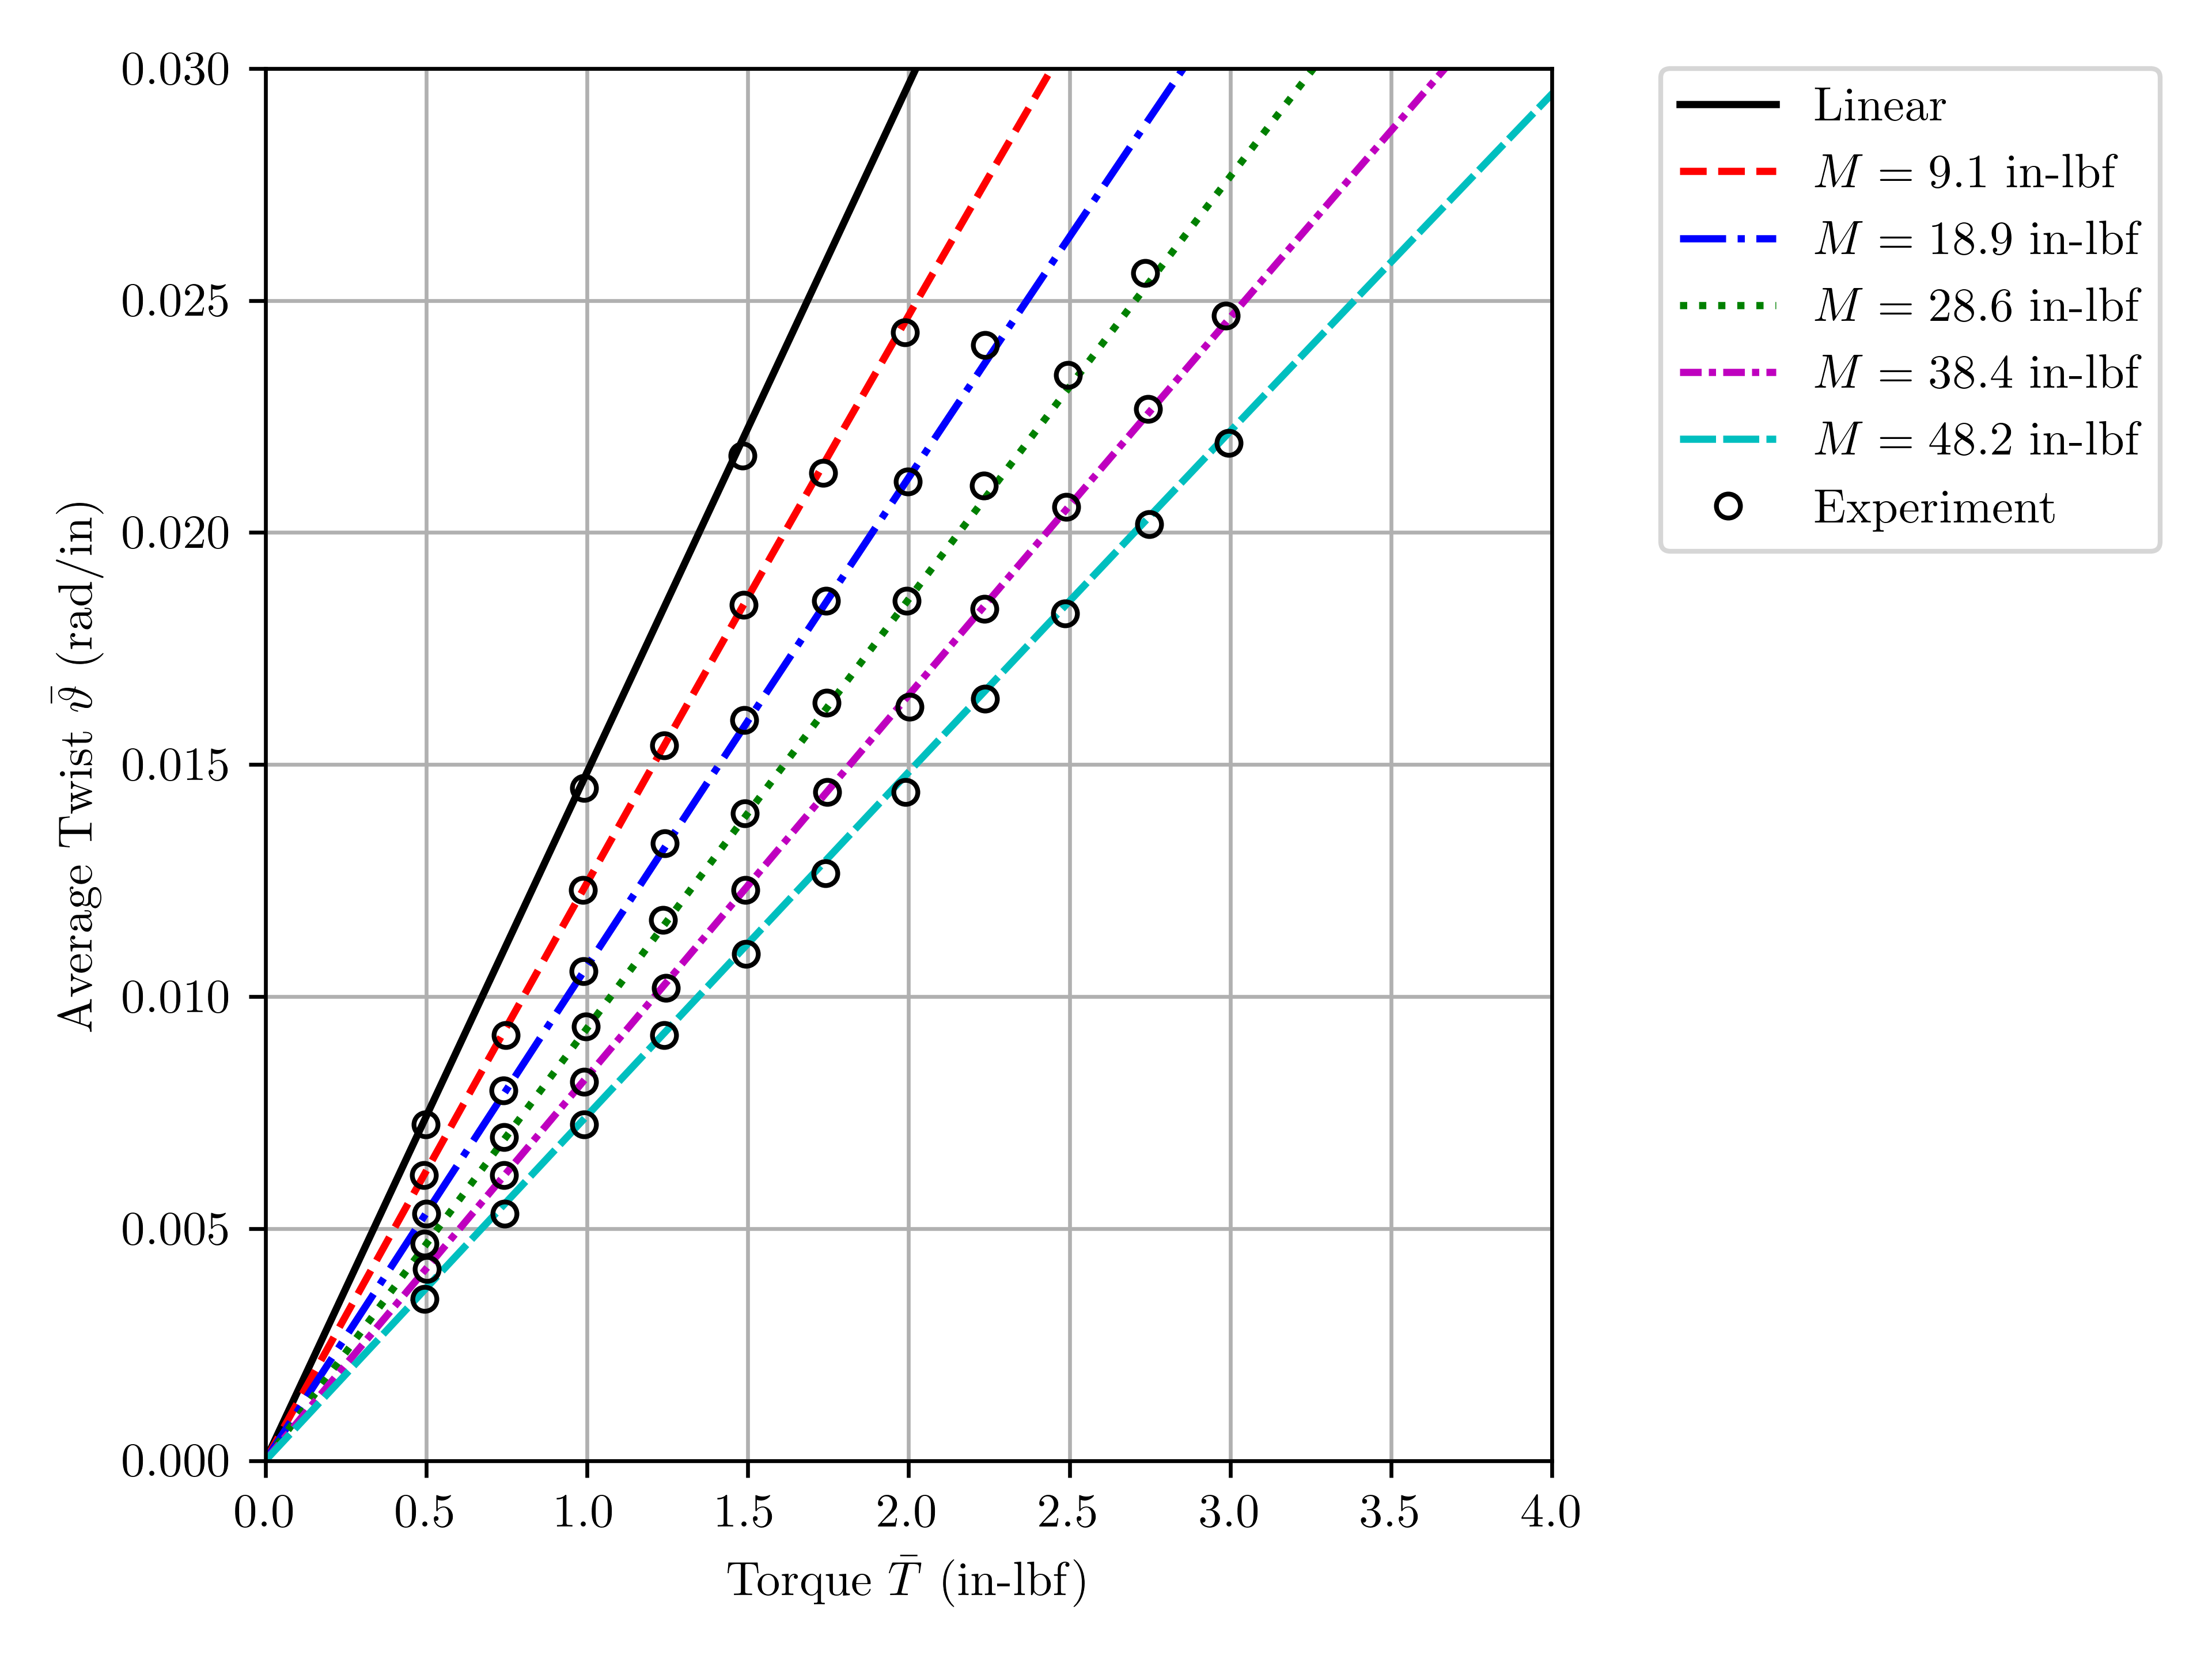
\includegraphics[width=\linewidth]{Examples/frame-1041/img/frame-1041-solution.png}
    \end{subfigure}
    \caption{Model for Example~\ref{sec:frame-0002}.}
    \label{fig:frame-0002}
\end{figure}

\subparagraph{Context.} 
This example extends the analysis of Example~\ref{sec:frame-0001} to use a section discretized by fibers. 
In the finite element kernel the section is not provided with any geometry-specific data apart from the general data described in Box~\ref{box:prep}.
The proposed compositional framework is employed to compute response gradients with respect to geometric parameters of interest. 

\subparagraph{Setup.}
The cantilever of \cref{fig:frame-0002} is loaded by a transverse tip force $\bar{F}$. 
The  cross-section is a solid rectangle of width $b$ and depth $d$. 

The cross-section is
represented by a grid of $N$~integration points, each characterized by a location $\bm{r}_k \in\Section$ and weight $A_k$.

The host parameters are the input data of the section (Box~\ref{box:prep}):
\begin{equation*}
\corey = \bigl(L,\; E,\; \bm{r}_1,\, A_1,\;\ldots,\;
               \bm{r}_N,\, A_N\bigr)
\;\in\; \mathbb{R}^{2+3N},
\end{equation*}
where $E$ is Young's modulus. 
Direct differentiation delivers $\partial u/\partial y_i$, where $u$ is the transverse tip displacement. 
%
The analyst, however, is interested in the dependence of~$u$ on the
section geometry:
\begin{equation}\label{eq:example-host}
\haty = (L,\; E,\; b,\; d) \;\in\; \mathbb{R}^{4}.
\end{equation}

Thus the parameter map~$\ParameterMap$ is 
\[
\ParameterMap(\HostParameters)
=
\bigl(
L,
E,
\mathcal F(d,b)
\bigr),
\]
where \(\mathcal F(d,b)\) generates a fiber discretization from geometric dimensions. 
Given a regular $n_x \times n_y$ grid over the rectangle
$[-b/2,\,b/2]\times[-d/2,\,d/2]$, the fiber coordinates and areas
are deterministic, differentiable functions of~$b$ and~$d$:
\begin{equation*}
    (b,\,d) \;\xmapsto{\;\mathcal{F}\;}\;
    \bigl\{(y_k,\, z_k,\, A_k)\bigr\}_{k=1}^{N}.
\end{equation*}

% \paragraph{End-to-end gradient.}
Composing $\Mmap$ with $\Ymap$ and applying the chain rule yields the
sensitivity of the tip displacement to the section depth:
\begin{equation*}
    \frac{\partial u}{\partial d}
    = \sum_{k=1}^{N}
      \biggl(
        \frac{\partial u}{\partial y_k}\,\frac{\partial y_k}{\partial d}
      + \frac{\partial u}{\partial z_k}\,\frac{\partial z_k}{\partial d}
      + \frac{\partial u}{\partial A_k}\,\frac{\partial A_k}{\partial d}
      \biggr),
\end{equation*}
where the terms $\partial u/\partial y_k$,
$\partial u/\partial z_k$, $\partial u/\partial A_k$ are provided by
the DDM inside the kernel, and the terms
$\partial y_k/\partial d$, $\partial z_k/\partial d$,
$\partial A_k/\partial d$ are computed by \autodiff{} of the parameter map $\Ymap$.

The analytic solution is
\begin{equation*}
    u = \frac{\bar{F} L^{3}}{3\,E\,I_y} + \frac{\bar{F}\,L}{G\,A},
\end{equation*}
where the second moment of area is $I_y = b\,d^{3}/12$  and
$G$ is the shear modulus.  
The derivative with respect to the depth $d$ is
\begin{equation*}
% \label{eq:example-exact-deriv}
    \frac{\partial u}{\partial d}
    % = \frac{\partial u}{\partial I_y}\,\frac{\partial I_y}{\partial d}
    % + \frac{\partial u}{\partial A}\,\frac{\partial A}{\partial d}
    = -\frac{\bar{F} L^{3}}{3\,E\,I_y^{2}}\;\frac{b\,d^{2}}{4}
      -\frac{\bar{F}\,L}{G\,A^{2}}\;b,
\end{equation*}
and serves as a verification target.

\subparagraph{Result.}
The composed numerical gradient
$\partial u/\partial d$ computed through the framework agrees with
this expression to the precision of the fiber discretisation.

